%----------------------------------------------------------------------------------------
%	PACKAGES AND THEMES
%----------------------------------------------------------------------------------------

\documentclass{beamer}

\mode<presentation> {

% The Beamer class comes with a number of default slide themes
% which change the colors and layouts of slides. Below this is a list
% of all the themes, uncomment each in turn to see what they look like.

%\usetheme{default}
%\usetheme{AnnArbor}
%\usetheme{Antibes}
%\usetheme{Bergen}
%\usetheme{Berkeley}
%\usetheme{Berlin}
%\usetheme{Boadilla}
%\usetheme{CambridgeUS}
\usetheme{Copenhagen}
%\usetheme{Darmstadt}
%\usetheme{Dresden}
%\usetheme{Frankfurt}
%\usetheme{Goettingen}
%\usetheme{Hannover}
%\usetheme{Ilmenau}
%\usetheme{JuanLesPins}
%\usetheme{Luebeck}
%\usetheme{Madrid}
%\usetheme{Malmoe}
%\usetheme{Marburg}
%\usetheme{Montpellier}
%\usetheme{PaloAlto}
%\usetheme{Pittsburgh}
%\usetheme{Rochester}
%\usetheme{Singapore}
%\usetheme{Szeged}
%\usetheme{Warsaw}

% As well as themes, the Beamer class has a number of color themes
% for any slide theme. Uncomment each of these in turn to see how it
% changes the colors of your current slide theme.

%\usecolortheme{albatross}
%\usecolortheme{beaver}
%\usecolortheme{beetle}
%\usecolortheme{crane}
%\usecolortheme{dolphin}
%\usecolortheme{dove}
%\usecolortheme{fly}
\usecolortheme{lily}
%\usecolortheme{orchid}
%\usecolortheme{rose}
%\usecolortheme{seagull}
%\usecolortheme{seahorse}
%\usecolortheme{whale}
%\usecolortheme{wolverine}

%\setbeamertemplate{footline} % To remove the footer line in all slides uncomment this line
%\setbeamertemplate{footline}[page number] % To replace the footer line in all slides with a simple slide count uncomment this line

%\setbeamertemplate{navigation symbols}{} % To remove the navigation symbols from the bottom of all slides uncomment this line
}

\usepackage{graphicx} % Allows including images
\usepackage{booktabs} % Allows the use of \toprule, \midrule and \bottomrule in tables
\usepackage[utf8]{inputenc}
\usepackage[T1]{fontenc}
\usepackage{amsmath}
\usepackage{multicol}

\usepackage{color}

\usepackage{url}

\usepackage{subfigure}
\usepackage{hyperref}

\usepackage{listings}
\usepackage{qvt}


\usepackage{mdframed}


\usepackage{pifont}% http://ctan.org/pkg/pifont
\newcommand{\cmark}{\ding{51}}%
\newcommand{\xmark}{\ding{55}}%

\renewcommand{\raggedright}{\leftskip=0pt \rightskip=0pt plus 0cm}

%----------------------------------------------------------------------------------------
%	TITLE PAGE
%----------------------------------------------------------------------------------------

\title[Comparing BX Tools with Examples]{Comparing BX Tools with Examples\\ } % The short title appears at the bottom of every slide, the full title is only on the title page
 
%\subtitle{FATBIT Workshop, Braga}

\author{	
FATBIT Workshop, Braga
} % Your name


\institute[DI.UM] % Your institution as it will appear on the bottom of every slide, may be shorthand to save space
{
HASLab, University of Minho \\ % Your institution for the title page
}
\date{October 3, 2013} % Date, can be changed to a custom date

\begin{document}

\begin{frame}
\titlepage % Print the title page as the first slide
\end{frame}

%\begin{frame}
%\frametitle{Overview} % Table of contents slide, comment this block out to remove it
%\tableofcontents % Throughout your presentation, if you choose to use \section{} and \subsection{} commands, these will automatically be printed on this slide as an overview of your presentation
%\end{frame}






%----------------------------------------------------------------------------------------
%	PRESENTATION SLIDES
%----------------------------------------------------------------------------------------


% Motivation ------------------------------------
\section{Motivation}

\begin{frame}
\frametitle{Motivation}

\begin{itemize}

\item \textbf{\textit{BX} Tools} comparisons are rare and lack \textbf{practical contexts}

\item potential users need \textbf{common comparison criteria/scenarios}

\end{itemize}

~\\

\begin{center}
assessment driven by \textbf{case studies}\\
 =\\
\textbf{pragmatic differentiation factor}
\end{center}


\end{frame}



% Approach ------------------------------------
\section{Approach}
\begin{frame}
\frametitle{Approach}

\begin{itemize}

\item elaborate \textbf{case studies} {\small (\textit{Metamodel} + \textit{Consistency Relation})}
 
\item choose different \textbf{\textit{BX} tools }

\item assess tool \textbf{expressiveness} and \textbf{efficiency}

\item assess transformations results against some \textbf{properties}


\end{itemize}

\end{frame}


% Tools to assess ------------------------------------
\section{Some tools to assess}
\begin{frame}
\frametitle{Some tools to assess}
\begin{footnotesize}
\textit{Tools}
\begin{itemize}
\item \textit{\textbf{eMoflon}} \cite{eMoflon}

\item \textit{\textbf{echo}} \cite{echotool}

\item \textit{GRoundTram} \cite{GRoundTram}
 
\item \textit{ModelMorf} \cite{ModelMorf}

\item \textit{Medini} \cite{medini}

\item \textit{focal} \cite{focal}
\end{itemize}
\textit{Properties}
\begin{itemize}
\item \textit{\textbf{correct}} \cite{Perdita1}\quad {\tiny $\forall m \in M \enskip \forall n \in N \qquad R(m,\overrightarrow{R}(m,n)) \enskip \land \enskip R(\overleftarrow{R}(m,n),n)$ }

\item \textit{\textbf{hippocratic}} \cite{Perdita1} \enskip {\tiny
$\forall m \in M \enskip \forall n \in N \quad R(m,n) \implies \overrightarrow{R}(m,n)=n \enskip \land \enskip \overleftarrow{R}(m,n)=m$ }

\item \textit{undoable} \cite{Perdita2}

\item \textit{history-ignorant} \cite{Perdita2}

\item \textit{simply-matching} \cite{Perdita2}

\item \textit{matching} \cite{Perdita2}

\item \textit{least-change} \cite{echo}
\end{itemize}
\end{footnotesize}

\end{frame}


% Case Studies ------------------------------------



% Bijection ------------------------------------

\section{Case Studies}

\subsection{Bijection}

\begin{frame}
\frametitle{\textbf{Bijection} - \textbf{Metamodel}}

\begin{figure}[ht]
    \centering
    \mbox{\subfigure[M]{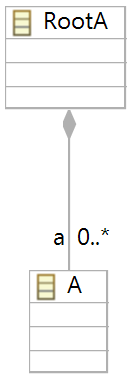
\includegraphics[scale=0.32]{printscreens/MMA.png}}\qquad\qquad
          \subfigure[N]{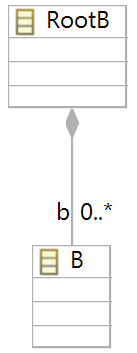
\includegraphics[scale=0.35]{printscreens/MMB.png}}
          }
    \caption{Metamodels}
    \label{fig:Meta}
\end{figure}

\end{frame}

\begin{frame}
\frametitle{Bijection - \textbf{Consistency Relation}}

\textbf{Type:} Bijection (Total Deterministic (\textit{TD})) -  $one <> one$\\

For every $M$ instance there
exists exactly one $N$ instance such that both are related by $R$ (and vice versa).


\begin{center}
\begin{tabular}{| c | c | c | c | c | }
  \hline                        
   & injective & entire & simple & surjective \\
  \hline 
  $R$ & \cmark & \cmark & \cmark & \cmark\\
  \hline  
\end{tabular}
\end{center}


\textbf{Definition}\\

For every \textit{A} in \textit{RootA} there
exists \textbf{exactly one} \textit{B} in \textit{RootB} (and vice versa).

%\footnote{Consider there exists only one \textit{World} and one \textit{Company} as containers. Actually they were only defined since \textit{Ecore} forces us to choose an instance root element, and nor \textit{Person} nor \textit{Employee} was an option since we want to model instances with multiple of these elements.}.

\end{frame}


% eMoflon ------------------------------------
\begin{frame}
\frametitle{Bijection - \textbf{Metamodel} - \textbf{\textit{\textcolor{orange}{eMoflon}}}}

\textit{Specification environment}: \textit{Enterprise Architect}

\begin{figure}[ht]
    \centering
    \mbox{\subfigure[$M$]{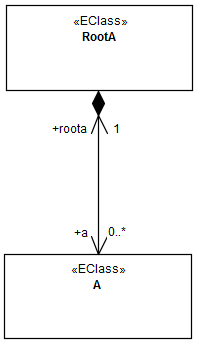
\includegraphics[scale=0.325]{printscreens/ea-MMA.png}}\qquad\qquad
          \subfigure[$N$]{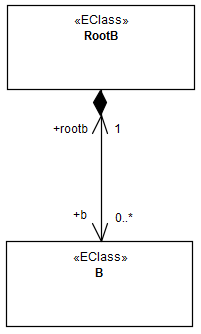
\includegraphics[scale=0.33]{printscreens/ea-MMB.png}}
          }
    \caption{Metamodels modelled as \textit{EA Ecore Diagrams}}
    \label{fig:ea-MMS}
\end{figure}

\end{frame}


\begin{frame}
\frametitle{Bijection - \textbf{Consistency Relation} - \textbf{\textit{\textcolor{orange}{eMoflon}}}}

\begin{figure}[ht]
  \centering 
  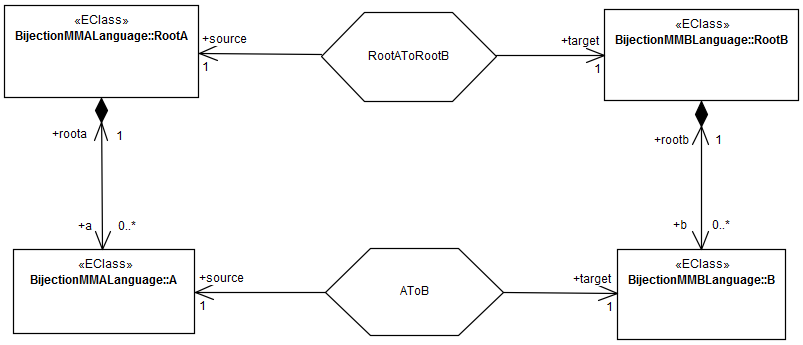
\includegraphics[scale=0.35]{printscreens/ea-MMAToMMB.png}
  \caption{\textit{TGG Schema Diagram}}
  \label{fig:ea-MMAToMMB}
\end{figure}

\end{frame}

\begin{frame}
\frametitle{Bijection - \textbf{Consistency Relation} - \textbf{\textit{\textcolor{orange}{eMoflon}}}}

\begin{figure}[ht]
  \centering 
  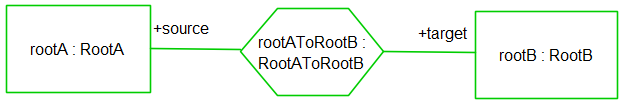
\includegraphics[scale=0.5]{printscreens/ea-RootAToRootB-rule.png}
  \caption{\textit{TGG Rule Diagram} - RootAToRootB}
  \label{fig:ea-RootAToRootB-rule}
\end{figure}

\end{frame}

\begin{frame}
\frametitle{Bijection - \textbf{Consistency Relation} - \textbf{\textit{\textcolor{orange}{eMoflon}}}}

\begin{figure}[ht]
  \centering 
  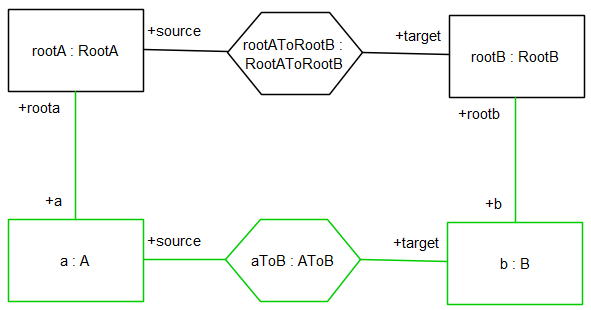
\includegraphics[scale=0.5]{printscreens/ea-AToB-rule.png}
  \caption{\textit{TGG Rule Diagram} - AToB}
  \label{fig:ea-AToB-rule}
\end{figure}

\end{frame}

\begin{frame}
\frametitle{Bijection - \textbf{Transformations} - \textbf{\textit{\textcolor{orange}{eMoflon}}}}
%T1 - \nameref{sec:one-person} / \nameref{sec:two-employees} 
\begin{figure}[ht]
\begin{mdframed}
    \centering
    \[ \mbox{\subfigure[$m$]{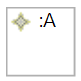
\includegraphics[scale=0.35]{printscreens/inst-oneA.png}}\qquad\qquad\qquad\qquad
          \subfigure[$n$]{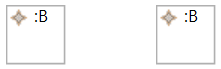
\includegraphics[scale=0.42]{printscreens/inst-twoBs.png}}
          } \]
\end{mdframed}
    \label{fig:T1}
\end{figure}

\begin{center}
$\overrightarrow{R}$
\end{center}

\begin{figure}[ht]
    \centering
    \mbox{
%    \subfigure[$m$]{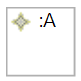
\includegraphics[scale=0.35]{printscreens/inst-oneA.png}}
          \subfigure[$n'$]{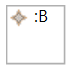
\includegraphics[scale=0.4]{printscreens/inst-oneB.png}}
          }
    \label{fig:T1}
\end{figure}


\end{frame}

\begin{frame}
\frametitle{Bijection - \textbf{Transformations} - \textbf{\textit{\textcolor{orange}{eMoflon}}}}
%T2 - \nameref{sec:one-person} / \nameref{sec:two-employees} 
\begin{figure}[ht]
\begin{mdframed}
    \centering
    \mbox{\subfigure[$m$]{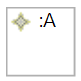
\includegraphics[scale=0.35]{printscreens/inst-oneA.png}}\qquad\qquad\qquad
          \subfigure[$n$]{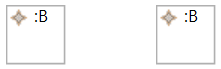
\includegraphics[scale=0.42]{printscreens/inst-twoBs.png}}
          }
\end{mdframed}          
    \label{fig:T1}
\end{figure}

\begin{center}
$\overleftarrow{R}$
\end{center}

\begin{figure}[ht]
    \centering
    \mbox{\subfigure[$m'$]{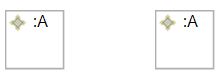
\includegraphics[scale=0.4]{printscreens/inst-twoAs.png}}
%          \subfigure[$n$]{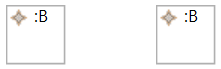
\includegraphics[scale=0.4]{printscreens/inst-twoBs.png}}
          }
    \label{fig:T2}
\end{figure}

\end{frame}

\begin{frame}
\frametitle{Bijection - \textbf{Transformations} - \textbf{\textit{\textcolor{orange}{eMoflon}}}}
%T3 - \nameref{sec:two-persons} / \nameref{sec:two-employees}
\begin{figure}[ht]
\begin{mdframed}
    \centering
    \mbox{\subfigure[$m$]{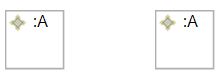
\includegraphics[scale=0.4]{printscreens/inst-twoAs.png}}\qquad\qquad\qquad
          \subfigure[$n$]{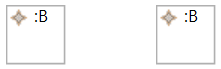
\includegraphics[scale=0.4]{printscreens/inst-twoBs.png}}
          }
\end{mdframed}          
    \label{fig:T1}
\end{figure}

\begin{center}
$\overrightarrow{R}$
\end{center}

\begin{figure}[ht]
    \centering
    \mbox{
%    \subfigure[$m$]{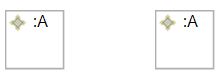
\includegraphics[scale=0.4]{printscreens/inst-twoAs.png}}
	\subfigure[$n'$]{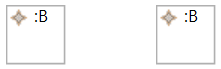
\includegraphics[scale=0.4]{printscreens/inst-twoBs.png}}
          }
    \label{fig:T3}
\end{figure}

\end{frame}

\begin{frame}
\frametitle{Bijection - \textbf{Transformations} - \textbf{\textit{\textcolor{orange}{eMoflon}}}}
%T4 - \nameref{sec:one-person} / \nameref{sec:no-employees}
\begin{figure}[ht]
\begin{mdframed}
    \centering
    \mbox{\subfigure[$m$]{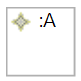
\includegraphics[scale=0.4]{printscreens/inst-oneA.png}}\qquad\qquad\qquad
          \subfigure[$n$]{
\includegraphics[scale=0.15]{printscreens/bij-empty.png}}
          }
\end{mdframed}          
    \label{fig:T1}
\end{figure}

\begin{center}
$\overrightarrow{R}$
\end{center}

\begin{figure}[ht]
    \centering
    \mbox{
%    \subfigure[$m$]{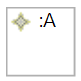
\includegraphics[scale=0.4]{printscreens/inst-oneA.png}}
   \subfigure[$n'$]{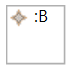
\includegraphics[scale=0.43]{printscreens/inst-oneB.png}}
          }
    \label{fig:T4}
\end{figure}

\end{frame}

\begin{frame}
\frametitle{Bijection - \textbf{Transformations} - \textbf{\textit{\textcolor{orange}{eMoflon}}}}
%T5 - \nameref{sec:no-persons} / \nameref{sec:no-employees}
\begin{figure}[ht]
\begin{mdframed}
    \centering
    \mbox{\subfigure[$m$]{
\includegraphics[scale=0.15]{printscreens/bij-empty.png}}\qquad\qquad\qquad
          \subfigure[$n$]{
\includegraphics[scale=0.15]{printscreens/bij-empty.png}}
          }
\end{mdframed}          
    \label{fig:T1}
\end{figure}
~\\

\begin{center}
$\overrightarrow{R}$
\end{center}

\begin{figure}[ht]
    \centering
    \mbox{
%    \subfigure[$m$]{
\includegraphics[scale=0.15]{printscreens/bij-empty.png}}
   \subfigure[$n'$]{
\includegraphics[scale=0.15]{printscreens/bij-empty.png}}
          }
    \label{fig:T5}
\end{figure}

\end{frame}




\begin{frame}
\frametitle{Bijection - \textbf{Assessment} - \textbf{\textit{\textcolor{orange}{eMoflon}}}}

For \textbf{the previous test instances in particular} the tool was:

\begin{center}
\begin{tabular}{| r | c |}
  \hline                        
  correct & \cmark\\
  \hline
  hippocratic & \cmark\\
  \hline 
%  undoable & ?\\
%  \hline 
%  history-ignorant & ?\\
%  \hline 
%  simply-matching & ?\\
%  \hline 
%  matching & ?\\
%  \hline 
%  least-change & \cmark\\
%  \hline   
\end{tabular}
\end{center}

\end{frame}












% echo ------------------------------------
\begin{frame}
\frametitle{Bijection - \textbf{Metamodel} - \textbf{\textit{\textcolor{green}{echo}}}}

\textit{Specification environment}: \textit{ Eclipse Modeling Tools}

\begin{figure}[ht]
    \centering
    \mbox{\subfigure[M]{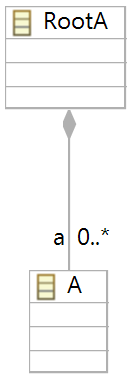
\includegraphics[scale=0.32]{printscreens/MMA.png}}\qquad\qquad
          \subfigure[N]{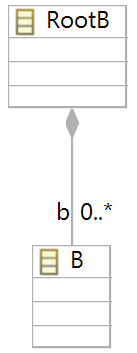
\includegraphics[scale=0.35]{printscreens/MMB.png}}
          }
    \caption{Metamodels}
    \label{fig:Meta}
\end{figure}

\end{frame}


\begin{frame}[fragile]
\frametitle{Bijection - \textbf{Consistency Relation} - \textbf{\textit{\textcolor{green}{echo}}}}

\begin{lstlisting}[language=QVT]
transformation a2b (as : A, bs : B) {
  top relation R2R { 
    domain as ra:RootA {};
    domain bs rb:RootB {};
    where { ra.as->size() = rb.bs->size(); } // not suitable QVT
  }
}
\end{lstlisting}

\end{frame}


\begin{frame}
\frametitle{Bijection - \textbf{Transformations} - \textbf{\textit{\textcolor{green}{echo}}}}

\begin{center}
\textit{same results as with eMoflon}
\end{center}

\end{frame}


\begin{frame}
\frametitle{Bijection - \textbf{Assessment} - \textbf{\textit{\textcolor{green}{echo}}}}

For \textbf{the previous test instances in particular} the tool was:

\begin{center}
\begin{tabular}{| r | c |}
  \hline                        
  correct & \cmark\\
  \hline
  hippocratic & \cmark\\
  \hline 
%  undoable & X\\
%  \hline 
%  history-ignorant & ?\\
%  \hline 
%  simply-matching & ?\\
%  \hline 
%  matching & ?\\
%  \hline 
%  least-change & \cmark\\
%  \hline   
\end{tabular}
\end{center}

\end{frame}

















% uniNDTotal -----------------------------------------------------

\subsection{uniNDTotal}

\begin{frame}
\frametitle{\textbf{uniNDTotal} - \textbf{Metamodel}}

\begin{figure}[ht]
    \centering
    \mbox{\subfigure[M]{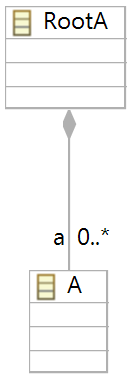
\includegraphics[scale=0.32]{printscreens/MMA.png}}\qquad\qquad
          \subfigure[N]{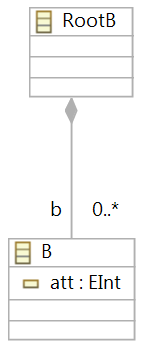
\includegraphics[scale=0.35]{printscreens/MMBatt.png}}
          }
    \caption{Metamodels}
    \label{fig:Meta}
\end{figure}

\end{frame}

\begin{frame}
\frametitle{uniNDTotal - \textbf{Consistency Relation}}

\textbf{Type:} \textit{Non Deterministic (only unidirectionally) Total (uniNDTotal)} - $one <> some$\\

~\\
For every $M$ instance there
exists \textbf{one} $N$ instance such that both are related by $R$;

For every $N$ instance there
exists \textbf{exactly one} $M$ instance such that both are related by $R$.

\begin{center}
\begin{tabular}{| c | c | c | c | c | }
  \hline                        
   & injective & entire & simple & surjective \\
  \hline 
  $R$ & \cmark & \cmark & X & \cmark\\
  \hline  
\end{tabular}
\end{center}


\textbf{Definition}\\

For every \textit{A} in \textit{RootA} there
exists \textbf{one} \textit{B} in \textit{RootB};

%\footnote{This direction is non deterministic since any \textit{B} is consistent regardless of its attribute value.}

For every \textit{B} in \textit{RootB} there
exists \textbf{exactly one} \textit{A} in \textit{RootA}.

\end{frame}


% eMoflon ------------------------------------
\begin{frame}
\frametitle{uniNDTotal - \textbf{Metamodel} - \textbf{\textit{\textcolor{orange}{eMoflon}}}}

\textit{Specification environment}: \textit{Enterprise Architect}

\begin{figure}[ht]
    \centering
    \mbox{\subfigure[$M$]{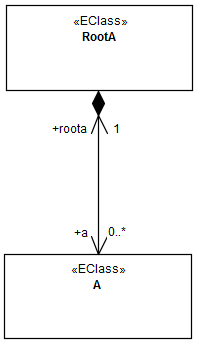
\includegraphics[scale=0.325]{printscreens/ea-MMA.png}}\qquad\qquad
          \subfigure[$N$]{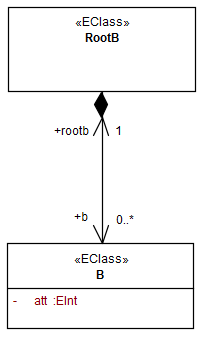
\includegraphics[scale=0.33]{printscreens/ea-MMBatt.png}}
          }
    \caption{Metamodels modelled as \textit{EA Ecore Diagrams}}
    \label{fig:ea-MMS}
\end{figure}

\end{frame}


\begin{frame}
\frametitle{uniNDTotal - \textbf{Consistency Relation} - \textbf{\textit{\textcolor{orange}{eMoflon}}}}

\begin{figure}[ht]
  \centering 
  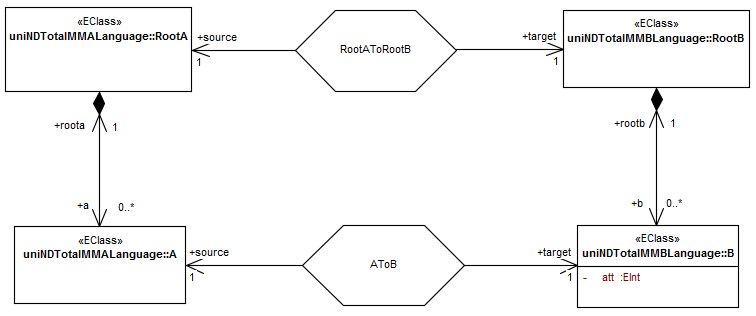
\includegraphics[scale=0.35]{printscreens/ea-MMAToMMBatt.png}
  \caption{\textit{TGG Schema Diagram}}
  \label{fig:ea-MMAToMMB}
\end{figure}

\end{frame}

\begin{frame}
\frametitle{uniNDTotal - \textbf{Consistency Relation} - \textbf{\textit{\textcolor{orange}{eMoflon}}}}

\begin{figure}[ht]
  \centering 
  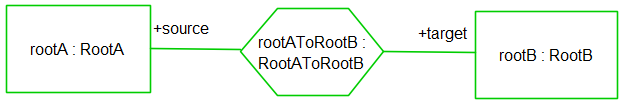
\includegraphics[scale=0.5]{printscreens/ea-RootAToRootB-rule.png}
  \caption{\textit{TGG Rule Diagram} - RootAToRootB}
  \label{fig:ea-RootAToRootB-rule}
\end{figure}

\end{frame}

\begin{frame}
\frametitle{uniNDTotal - \textbf{Consistency Relation} - \textbf{\textit{\textcolor{orange}{eMoflon}}}}

\begin{figure}[ht]
  \centering 
  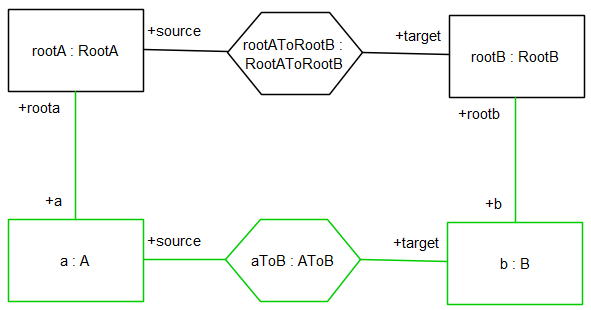
\includegraphics[scale=0.5]{printscreens/ea-AToB-rule.png}
  \caption{\textit{TGG Rule Diagram} - AToB}
  \label{fig:ea-AToB-rule}
\end{figure}

\end{frame}

\begin{frame}
\frametitle{uniNDTotal - \textbf{Transformations} - \textbf{\textit{\textcolor{orange}{eMoflon}}}}
%T1 - \nameref{sec:oneA} / \nameref{sec:oneBatt0}
\begin{figure}[ht]
\begin{mdframed}
    \centering
    \mbox{\subfigure[$m$]{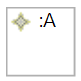
\includegraphics[scale=0.35]{printscreens/inst-oneA.png}}\qquad\qquad\qquad
          \subfigure[$n$]{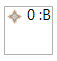
\includegraphics[scale=0.5]{printscreens/inst-oneBatt0.png}}
          }
\end{mdframed}          
    \label{fig:T1}
\end{figure}

\begin{center}
$\overrightarrow{R}$
\end{center}

\begin{figure}[ht]
    \centering
    \mbox{
%    \subfigure[$m$]{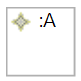
\includegraphics[scale=0.35]{printscreens/inst-oneA.png}}
    \subfigure[$n'$]{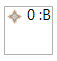
\includegraphics[scale=0.5]{printscreens/inst-oneBatt0.png}}
          }
    \label{fig:T1}
\end{figure}


\end{frame}

\begin{frame}
\frametitle{uniNDTotal - \textbf{Transformations} - \textbf{\textit{\textcolor{orange}{eMoflon}}}}
%T2 - \nameref{sec:noAs} / \nameref{sec:oneBatt15}
\begin{figure}[ht]
\begin{mdframed}
    \centering
    \mbox{\subfigure[$m$]{
\includegraphics[scale=0.15]{printscreens/bij-empty.png}}\qquad\qquad\qquad
          \subfigure[$n$]{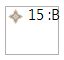
\includegraphics[scale=0.5]{printscreens/inst-oneBatt15.png}}
          }
\end{mdframed}          
    \label{fig:T1}
\end{figure}

\begin{center}
$\overleftarrow{R}$
\end{center}

\begin{figure}[ht]
    \centering
    \mbox{\subfigure[$m'$]{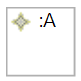
\includegraphics[scale=0.35]{printscreens/inst-oneA.png}}
%          \subfigure[$n$]{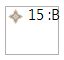
\includegraphics[scale=0.5]{printscreens/inst-oneBatt15.png}}
          }
    \label{fig:T2}
\end{figure}

\end{frame}

\begin{frame}
\frametitle{uniNDTotal - \textbf{Transformations} - \textbf{\textit{\textcolor{orange}{eMoflon}}}}
%T3 - \nameref{sec:oneA} / \nameref{sec:oneBatt15}
\begin{figure}[ht]
\begin{mdframed}
    \centering
    \mbox{\subfigure[$m$]{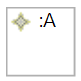
\includegraphics[scale=0.35]{printscreens/inst-oneA.png}}\qquad\qquad\qquad
          \subfigure[$n$]{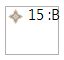
\includegraphics[scale=0.5]{printscreens/inst-oneBatt15.png}}
          }
\end{mdframed}          
    \label{fig:T1}
\end{figure}

\begin{center}
$\overrightarrow{R}$
\end{center}

\begin{figure}[ht]
    \centering
    \mbox{
%    \subfigure[$m$]{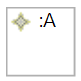
\includegraphics[scale=0.35]{printscreens/inst-oneA.png}}
	\subfigure[$n'$]{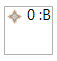
\includegraphics[scale=0.5]{printscreens/inst-oneBatt0.png}}
          }
    \label{fig:T3}
\end{figure}

\end{frame}



\begin{frame}
\frametitle{uniNDTotal - \textbf{Assessment} - \textbf{\textit{\textcolor{orange}{eMoflon}}}}

For \textbf{the previous test instances in particular} the tool was:

\begin{center}
\begin{tabular}{| r | c |}
  \hline                        
  correct & \cmark\\
  \hline
  hippocratic & X \\
  \hline 
%  undoable & ?\\
%  \hline 
%  history-ignorant & ?\\
%  \hline 
%  simply-matching & ?\\
%  \hline 
%  matching & ?\\
%  \hline 
%  least-change & X\\
%  \hline   
\end{tabular}
\end{center}

\end{frame}

















% echo ------------------------------------
\begin{frame}
\frametitle{uniNDTotal - \textbf{Metamodel} - \textbf{\textit{\textcolor{green}{echo}}}}

\textit{Specification environment}: \textit{Eclipse Modeling Tools}

\begin{figure}[ht]
    \centering
    \mbox{\subfigure[M]{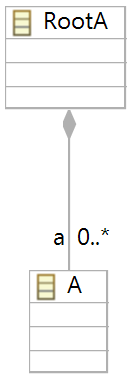
\includegraphics[scale=0.32]{printscreens/MMA.png}}\qquad\qquad
          \subfigure[N]{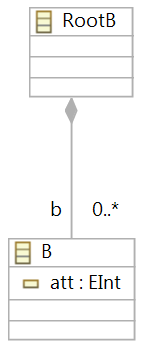
\includegraphics[scale=0.35]{printscreens/MMBatt.png}}
          }
    \caption{Metamodels}
    \label{fig:Meta}
\end{figure}

\end{frame}


\begin{frame}[fragile]
\frametitle{uniNDTotal - \textbf{Consistency Relation} - \textbf{\textit{\textcolor{green}{echo}}}}

\begin{lstlisting}[language=QVT]
transformation a2b (as : A, bs : B) {
  top relation R2R { 
    domain as ra:RootA {};
    domain bs rb:RootB {};
    where { ra.as->size() = rb.bs->size(); }
  }
}
\end{lstlisting}



\end{frame}


\begin{frame}
\frametitle{uniNDTotal - \textbf{Transformations} - \textbf{\textit{\textcolor{green}{echo}}}}
%T1 - \nameref{sec:oneA} / \nameref{sec:oneBatt0}
\begin{figure}[ht]
\begin{mdframed}
    \centering
    \mbox{\subfigure[$m$]{\includegraphics[scale=0.35]{printscreens/inst-oneA.png}}\qquad\qquad\qquad
          \subfigure[$n$]{\includegraphics[scale=0.5]{printscreens/inst-oneBatt0.png}}
          }
\end{mdframed}          
    \label{fig:T1}
\end{figure}

\begin{center}
$\overrightarrow{R}$
\end{center}

\begin{figure}[ht]
    \centering
    \mbox{
%    \subfigure[$m$]{\includegraphics[scale=0.35]{printscreens/inst-oneA.png}}
	\subfigure[$n'$]{\includegraphics[scale=0.5]{printscreens/inst-oneBatt0.png}}
          }
    \label{fig:T1}
\end{figure}


\end{frame}

\begin{frame}
\frametitle{uniNDTotal - \textbf{Transformations} - \textbf{\textit{\textcolor{green}{echo}}}}
%T2 - \nameref{sec:noAs} / \nameref{sec:oneBatt15}
\begin{figure}[ht]
\begin{mdframed}
    \centering
    \mbox{\subfigure[$m$]{\includegraphics[scale=0.15]{printscreens/bij-empty.png}}\qquad\qquad\qquad
          \subfigure[$n$]{\includegraphics[scale=0.5]{printscreens/inst-oneBatt15.png}}
          }
\end{mdframed}          
    \label{fig:T1}
\end{figure}

\begin{center}
$\overleftarrow{R}$
\end{center}

\begin{figure}[ht]
    \centering
    \mbox{\subfigure[$m'$]{\includegraphics[scale=0.35]{printscreens/inst-oneA.png}}
%          \subfigure[$n$]{\includegraphics[scale=0.5]{printscreens/inst-oneBatt15.png}}
          }
    \label{fig:T2}
\end{figure}

\end{frame}

\begin{frame}
\frametitle{uniNDTotal - \textbf{Transformations} - \textbf{\textit{\textcolor{green}{echo}}}}
%T3 - \nameref{sec:oneA} / \nameref{sec:oneBatt15}
\begin{figure}[ht]
\begin{mdframed}
    \centering
    \mbox{\subfigure[$m$]{\includegraphics[scale=0.35]{printscreens/inst-oneA.png}}\qquad\qquad\qquad
          \subfigure[$n$]{\includegraphics[scale=0.5]{printscreens/inst-oneBatt15.png}}
          }
\end{mdframed}          
    \label{fig:T1}
\end{figure}

\begin{center}
$\overrightarrow{R}$
\end{center}

\begin{figure}[ht]
    \centering
    \mbox{
%    \subfigure[$m$]{\includegraphics[scale=0.35]{printscreens/inst-oneA.png}}
	\subfigure[$n'$]{\includegraphics[scale=0.5]{printscreens/inst-oneBatt15.png}}
          }
    \label{fig:T3}
\end{figure}

\end{frame}


\begin{frame}
\frametitle{uniNDTotal - \textbf{Assessment} - \textbf{\textit{\textcolor{green}{echo}}}}

For \textbf{the previous test instances in particular} the tool was:

\begin{center}
\begin{tabular}{| r | c |}
  \hline                        
  correct & \cmark\\
  \hline
  hippocratic & \cmark\\
  \hline 
%  undoable & ?\\
%  \hline 
%  history-ignorant & ?\\
%  \hline 
%  simply-matching & ?\\
%  \hline 
%  matching & ?\\
%  \hline 
%  least-change & \cmark\\
%  \hline   
\end{tabular}
\end{center}

\end{frame}







% References ------------------------------------------------
\section{References}
\begin{frame}

\frametitle{References}


\begin{scriptsize}

\begin{thebibliography}{99} % Beamer does not support BibTeX so references must be inserted manually as below

\bibitem{Perdita1} Stevens, Perdita. "Bidirectional model transformations in QVT: Semantic issues and open questions." Model Driven Engineering Languages and Systems. Springer Berlin Heidelberg, 2007. 1-15.

\bibitem{Perdita2} Stevens, Perdita. "Observations relating to the equivalences induced on model sets by bidirectional transformations." Electronic Communications of the EASST 49 (2012).

\bibitem{echo} Macedo, Nuno, and Alcino Cunha. "Implementing QVT-R bidirectional model transformations using Alloy." Fundamental Approaches to Software Engineering. Springer Berlin Heidelberg, 2013. 297-311.

%------------------ tools

\bibitem{eMoflon} eMoflon - \url{http://www.moflon.org/}

\bibitem{echotool} echo - \url{https://github.com/haslab/echo}

\bibitem{GRoundTram} GRoundTram - \url{http://www.biglab.org/}

\bibitem{ModelMorf} ModelMorf - \url{http://www.tcs-trddc.com/}

\bibitem{medini} medini QVT - \url{http://projects.ikv.de/qvt}

\bibitem{focal} focal - \url{https://alliance.seas.upenn.edu/~harmony/old/}

\end{thebibliography}
\end{scriptsize}


\end{frame}



% Front Frame ------------------------------------------------

%\begin{frame}
%\titlepage
%\end{frame}

% End -------------------------------------------------------
% -------------------------------------------------------
% -------------------------------------------------------




\end{document} 
